\documentclass{article}

\usepackage{amsmath}
\usepackage{amssymb}
\usepackage{algorithm}
\usepackage[noend]{algpseudocode}		% for algorithms in pseudo code. Usage: \begin{algorithmic}
\usepackage{tikz}
\usepackage{subcaption}

\newcommand{\vecl}{\overrightarrow} % long vector for multiple characters
\newcommand{\ang}[1]{\measuredangle\left( #1 \right)}
\newcommand{\len}[1]{\left\lVert #1 \right\rVert}
\newcommand{\inta}[1]{\operatorname{int}\left( #1 \right)} % interior angle
\newcommand{\exta}[1]{\operatorname{ext}\left( #1 \right)} % exterior angle

\title{Determining the Convexity of any Polygon}
\author{Abraham Murciano}

\begin{document}
\maketitle

\section{Abstract}

This paper presents and proves the correctness of an algorithm which determines if a sequence of points in three-dimensional space forms a convex polygon or not. We will discuss simple concave polygons as well as complex (self intersecting) polygons. As an added bonus, we will be able to detect and reject any input whose vertices do not lie on a common plane.

\section{Definitions}

\begin{description}
	\item[Angle between vectors]
		The angle between two three-dimensional vectors \(\vec{u}\) and \(\vec{v}\), which we shall denote henceforth as \(\ang{\vec{u}, \vec{v}}\), is defined as follows.
		\begin{equation*}
			\ang{\vec{u}, \vec{v}} = \arccos \left( \frac{\vec{u} \cdot \vec{v}} {\len{\vec{u}} \cdot \len{\vec{v}}} \right)
		\end{equation*}
		It is important to note that \(\ang{\vec{u}, \vec{v}}\) is always between 0 and \(\pi\) radians. For any two vectors there are two angles between them, and the function \(\measuredangle\) always gives us the smaller of the two.

	\item[Polygon]
		A polygon is a \emph{plane} figure that is described by a finite number of straight line segments connected to form a closed circuit. The enclosed plane region, as well as the bounding circuit, is what we shall call a polygon.

	\item[Simple polygon]
		A simple polygon is a polygon whose bounding line segments do not intersect with each other.

	\item[Interior angle]
		For a simple polygon, an angle between two adjacent line segments is called an interior angle (or internal angle) if a point within the angle is in the interior of the polygon. A simple polygon has exactly one internal angle per vertex.

		We shall denote the interior angle at vertex \(Q\) as \(\inta{Q}\).

	\item[Exterior angle]
		If \(P\), \(Q\), and \(R\) are three consecutive vertices of a polygon (such that \(Q\) is in between \(P\) and \(R\)), the exterior angle of the polygon at a vertex \(Q\) is \(\exta{Q} = \ang{\vecl{PQ}, \vecl{QR}}\).

		Note, since the range of the function \(\measuredangle\) is \([0, \pi]\), by `exterior angle' we refer always (unless otherwise noted) to a positive angle.

	\item[Convex polygon]
		A polygon is convex if it is simple and all its interior angles are less than \(\pi\) radians.

	\item[Concave polygon]
		A polygon is concave if it is simple and not convex.

	\item[Complex polygon]
		A polygon is complex if it is not simple, i.e. if its edges intersect with each other. There is debate whether or not complex polygons are considered polygons, but for the purposes of this paper we shall refer to them as polygons.
\end{description}

\begin{figure}[htbp]
	\centering
	\begin{subfigure}{0.25\textwidth}
		\centering
		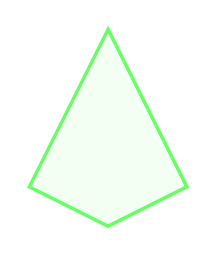
\begin{tikzpicture}
			\filldraw[color=green!60, fill=green!5, very thick] (0, 0) -- (1, -0.5) -- (2, 0) -- (1, 2) -- cycle;
		\end{tikzpicture}
		\caption{Convex}
	\end{subfigure}%
	\begin{subfigure}{0.25\textwidth}
		\centering
		
\begin{tikzpicture}
			\filldraw[color=orange!60, fill=orange!5, very thick] (0, 0) -- (1, 0.5) -- (2, 0) -- (1, 2.5) -- cycle;
		\end{tikzpicture}
		\caption{Concave}
	\end{subfigure}%
	\begin{subfigure}{0.25\textwidth}
		\centering
		
\begin{tikzpicture}
			\filldraw[color=red!60, fill=red!5, very thick] (0, 0) -- (2, 2.5) -- (0, 2.5) -- (2, 0) -- cycle;
		\end{tikzpicture}
		\caption{Complex}
	\end{subfigure}%
	\caption{Examples of different types of polygons.}
	\label{}
\end{figure}

\section{The Algorithm}

We will begin by explaining how the algorithm works, then presenting the algorithm at the end of this section.

\subsection{Input}

The algorithm accepts a sequence of points in three-dimensional space. The points, if they share a common plane, represent a polygon formed by constructing an edge between all adjacent vertices in the sequence and an additional edge between the first and last vertices.

\subsection{Output}

The algorithm returns True if the input forms a convex polygon, and False otherwise.

Some examples of when the input does not form a convex polygon are
\begin{itemize}
	\item if the points form a concave polygon,
	\item if the points form a complex polygon, and
	\item if the points do not share a common plane, and thus do not form a polygon at all.
\end{itemize}

\subsection{Processing}

The algorithm boils down to a single check. A sequence of vertices forms a simple convex polygon if and only if the sum of the exterior angles is equal to \(2\pi\). Formally, the algorithm checks if the following equation holds true, where \(V\) is the input sequence of vertices.

\begin{equation*}
	\sum_{v \in V} \exta{v} = 2\pi
\end{equation*}

\subsection{Pseudo Code}

The function \textsc{IsConvex} takes as input a sequence of points \(V\) and returns whether or not the points form a convex polygon.

\begin{algorithm}[htbp]
	\begin{algorithmic}
		\Function{IsConvex}{$V$}
		\If{\(|V| < 3\)}
		\Return False
		\EndIf
		\State \(s := 0\) \Comment{The sum of the exterior angles.}
		\For{\(i\) from 0 to \(|V| - 1\)}
		\State \(P := V_{i-1 \mod |V|}\) \Comment{The previous point.}
		\State \(Q := V_{i}\) \Comment{The current point.}
		\State \(R := V_{i+1 \mod |V|}\) \Comment{The next point.}
		\State \(s := s + \ang{\vecl{PQ}, \vecl{QR}}\) \Comment{Add the exterior angle of \(Q\).}
		\EndFor
		\State\Return \(s = 2\pi\)
		\EndFunction
	\end{algorithmic}
\end{algorithm}

\section{Proof of Correctness}

\subsection{Claim}

A sequence of vertices \(V\) forms a simple convex polygon if and only if the sum of the exterior angles is equal to \(2\pi\).

\subsection{Proof}

In order to prove our claim, we must prove (a) that if a polygon is simple then the sum of its exterior angles is equal to \(2\pi\), and (b) that if a sequence of points' angles sum to \(2\pi\), then it must form a convex polygon. We shall commence with the easier of the two.

\subsubsection{Convex Polygons' Exterior Angles Sum to \(2\pi\)}

\paragraph{Lemma 1.} If a polygon with \(n\) sides is convex, then we know that the sum of the interior angles must be \(\pi(n - 2)\). (Proof omitted.)

\paragraph{Lemma 2.} For every point on a convex polygon, the sum of the interior and exterior angles must be \(\pi\) radians. (Proof omitted.)

\paragraph{Proof.} Given a convex polygon with the sequence of vertices \(V\), by lemma 1 we can formulate \(|V|\) equations; one for each vertex \(v \in V\).
\begin{equation}
	\inta{v} + \exta{v} = \pi
\end{equation}

If we take the sum of all equations in this family of equations, we obtain the following equation.
\begin{equation}
	\sum_{v \in V} \inta{v} + \sum_{v \in V} \exta{v} = n\pi
\end{equation}
This can then be rearranged into the next equation.
\begin{equation}
	\sum_{v \in V} \exta{v} = n\pi - \sum_{v \in V} \inta{v}
\end{equation}
But by lemma 1, we know the sum of the interior angles of the convex polygon.
\begin{equation}
	\sum_{v \in V} \exta{v} = n\pi - \pi(n-2) = n\pi - n\pi + 2\pi = 2\pi
\end{equation}

\subsubsection{Only Convex Polygons' Angles Sum to \(2\pi\)}



\end{document}